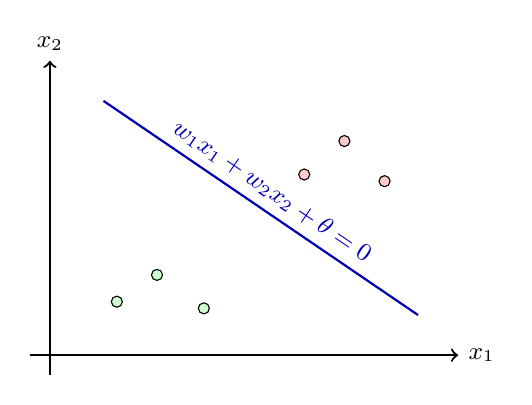
\begin{tikzpicture}[
    x=0.85cm,
    y=0.85cm,
    every node/.style={font=\small}
]

    \draw[->, thick] (-0.3,0) -- (6.1,0) node[right] {\(x_1\)};
    \draw[->, thick] (0,-0.3) -- (0,4.4) node[above] {\(x_2\)};

    \draw[thick, blue!70!black] (0.8,3.8) -- node[midway,above,sloped] {\(w_1x_1+w_2x_2+\theta=0\)} (5.5,0.6);

    \draw[fill=green!20] (1.0,0.8) circle (2pt);
    \draw[fill=green!20] (1.6,1.2) circle (2pt);
    \draw[fill=green!20] (2.3,0.7) circle (2pt);

    \draw[fill=red!20] (4.4,3.2) circle (2pt);
    \draw[fill=red!20] (5.0,2.6) circle (2pt);
    \draw[fill=red!20] (3.8,2.7) circle (2pt);

\end{tikzpicture}
